\documentclass[14pt]{extarticle}
\usepackage{graphicx}
\usepackage[T1]{fontenc} 

% Custom captions: 1 pav.
\usepackage{caption}
\captionsetup[figure]{labelformat=empty}
\renewcommand{\thefigure}{\arabic{figure} pav.}

% Turinys vietoj Contents
\renewcommand{\contentsname}{Turinys}

\begin{document}

% Titulinis
\begin{titlepage}
	\begin{center}
		
\includegraphics[width=5cm]{images/ktu_logo.png}

		\textbf{Kauno technologijos universitetas}

		Informatikos fakultetas

		\vspace{3cm}

		\textbf{Laboratorinis darbas Nr. 3}

		\vspace{0.5cm}
		T120B019 ŽMOGAUS-KOMPIUTERIO SĄSAJOS PROJEKTAVIMAS

	\end{center}

	\begin{flushright}

		\vfill

		\textbf{Arnas Bradauskas} \\
		\textbf{Ignas Survila} \\
		\textbf{Ignas Eismantas}

		Studentai

		\vspace{0.2cm}

		\textbf{asist. Ligita Zailskaitė-Jakštė}

		Dėstytojas

	\end{flushright}

	\begin{center}
		Kaunas, 2024
	\end{center}

\end{titlepage}

% Turinys
\tableofcontents

\clearpage

\section{Darbo tikslas}

Darbo tikslas: apibrėžti kuriamo IT produkto (informacinės sistemos, interneto svetainės arba
mobiliosios aplikacijos) sąsajos viziją. Produktas turi atitikti realių vartotojų poreikius ir
reikalavimus ir gali būti praktiškai įgyvendinamas. Darbe analizuojamas ir aprašomas kuriamo
produkto (sistemos) naudojimo kontekstas, suvokiant potencialių produkto naudotojų
poreikius ir galimas naudojimo problemas. Aprašomas produkto naudojimo tipinis scenarijus.

\clearpage

\section{Būsimos sistemos naudotojų grupės ir jų poreikiai}

\subsection{Pirminiai naudotojai (vyresnio amžiaus žmonės)}

\begin{itemize}
	\item Lengvai seka savo vaistų vartojimo tvarkaraštį
	\item Gauna priminimus apie vaistų vartojimo laiką
	\item Stebi likusių vaistų kiekį
	\item Paprastai registruoja naujus vaistus
\end{itemize}

\subsection{Antriniai naudotojai (šeimos nariai, globėjai)}

\begin{itemize}
	\item Stebi artimojo vaistų vartojimą
	\item Gauna pranešimus, jei vaistai nevartojami laiku
	\item Padeda tvarkyti vaistų sąrašą ir tvarkaraštį
\end{itemize}

\subsection{IT aptarnaujantis personalas}

\begin{itemize}
	\item Stebi ir tobulina sistemą
\end{itemize}

\clearpage

\section{Naudotojų grupių charakteristikos}

\subsection{Pirminiai naudotojai}

\begin{itemize}
	\item Amžius: 65+ metų
	\item IT patirtis: ribota, dažnai neturi daug patirties su išmaniaisiais įrenginiais
	\item Galimi apribojimai: regėjimo, klausos ar motorikos sutrikimai
\end{itemize}

\subsection{Antriniai naudotojai}

\begin{itemize}
	\item Amžius: įvairus, dažniausiai 30-60 metų
	\item IT patirtis: vidutinė
	\item Charakteristikos: rūpestingi, norintys padėti
\end{itemize}

\subsection{IT aptarnaujantis personalas}

\begin{itemize}
	\item Amžius: darbinis
	\item IT patirtis: aukšta
\end{itemize}

\clearpage

\section{Sąsajos veiklų ir jų konteksto aprašymai}

\begin{itemize}
	\item Fizinė aplinka: dažniausiai namų aplinka, gali būti prastas apšvietimas
	\item Socialinis kontekstas: svarbu užtikrinti privatumą ir duomenų saugumą
	\item Individualūs skirtumai: atsižvelgti į galimus regėjimo, klausos ar motorikos sutrikimus
\end{itemize}

\clearpage

\section{Naudotojų tikslai}

\begin{itemize}
	\item Laiku ir teisingai vartoti vaistus
	\item Išvengti vaistų praleidimo ar perdozavimo
	\item Lengvai sekti likusių vaistų kiekį
	\item Dalintis informacija su šeimos nariais ar gydytojais
\end{itemize}

\clearpage

\section{Užduočių analizė}

\begin{figure}[!htbp]
	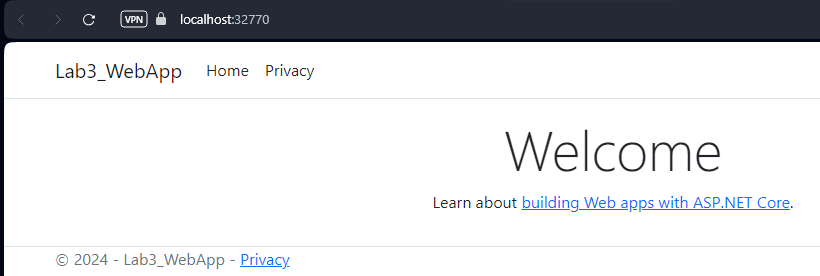
\includegraphics[width=5.5in]{images/flow.png}
	\caption{\thefigure\ User Flow diagrama.}
\end{figure}

\clearpage

\section{Tipinis naudojimosi scenarijus}

Ona (72 m.) turi vartoti tris skirtingus vaistus per dieną. Ji naudojasi "VaistuPriminimai" aplikacija:

8:00 ryto Ona gauna garsinį ir vizualinį priminimą apie rytinį vaistą.
Ji paima vaistą ir patvirtina jo suvartojimą aplikacijoje.
Aplikacija automatiškai atnaujina likusių vaistų kiekį.
14:00 ir 20:00 procesas kartojasi su kitais vaistais.
Vakare Ona peržiūri dienos suvestinę ir mato, kad suvartojo visus vaistus laiku.
Jos dukra, kuri taip pat turi prieigą prie Onos paskyros, patikrina mamos vaistų vartojimą ir jaučiasi rami.

\section{Sąsajų dizaino idėjos}

\begin{itemize}
	\item Didelis, aiškus šriftas ir ryškios, kontrastingos spalvos
	\item Paprastas, intuityvus meniu su dideliais mygtukais
	\item Galimybė naudoti balso komandas
	\item Aiškūs garsiniai ir vizualiniai priminimai
	\item Lengvai suprantamos piktogramos vaistams žymėti
\end{itemize}

\clearpage

\section{Sistemos sąsajų maketai}

 [Čia būtų įterpiami maketai, sukurti naudojant sąsajų prototipų kūrimo įrankį. Pagrindiniai maketai galėtų būti:

  Pagrindinis langas su dienos vaistų tvarkaraščiu
  Vaisto vartojimo patvirtinimo langas
  Vaistų sąrašo peržiūros ir redagavimo langas
  Priminimų nustatymų langas
  Pranešimų pavyzdys (pvz., priminimas apie vaisto vartojimą)]

\clearpage

\section{Išvados}

\begin{itemize}
	\item Išmokome analizuoti ir suprasti vyresnio amžiaus žmonių poreikius naudojant technologijas.
	\item Įgijome patirties kuriant vartotojo sąsają, pritaikytą specifinei vartotojų grupei.
	\item Patobulinome mobiliųjų aplikacijų projektavimo įgūdžius.
	\item Išmokome ieškoti kūrybiškų sprendimų kasdienėms vyresnio amžiaus žmonių problemoms.
\end{itemize}

\end{document}
